\section{Interactions Between Modules}\label{sec:interactions}

To provide a clearer view of the interactions among modules, this section
presents sequence diagrams illustrating the main interactions between system
components.

\figref{fig:mining-sequence} shows the UML sequence diagram detailing the
interactions that occur when a \code{Miner} successfully mines a new block.

\figref{fig:txgen-sequence} illustrates the sequence of interactions involved
in creating a new transaction.

\begin{sidewaysfigure}
	\centering
	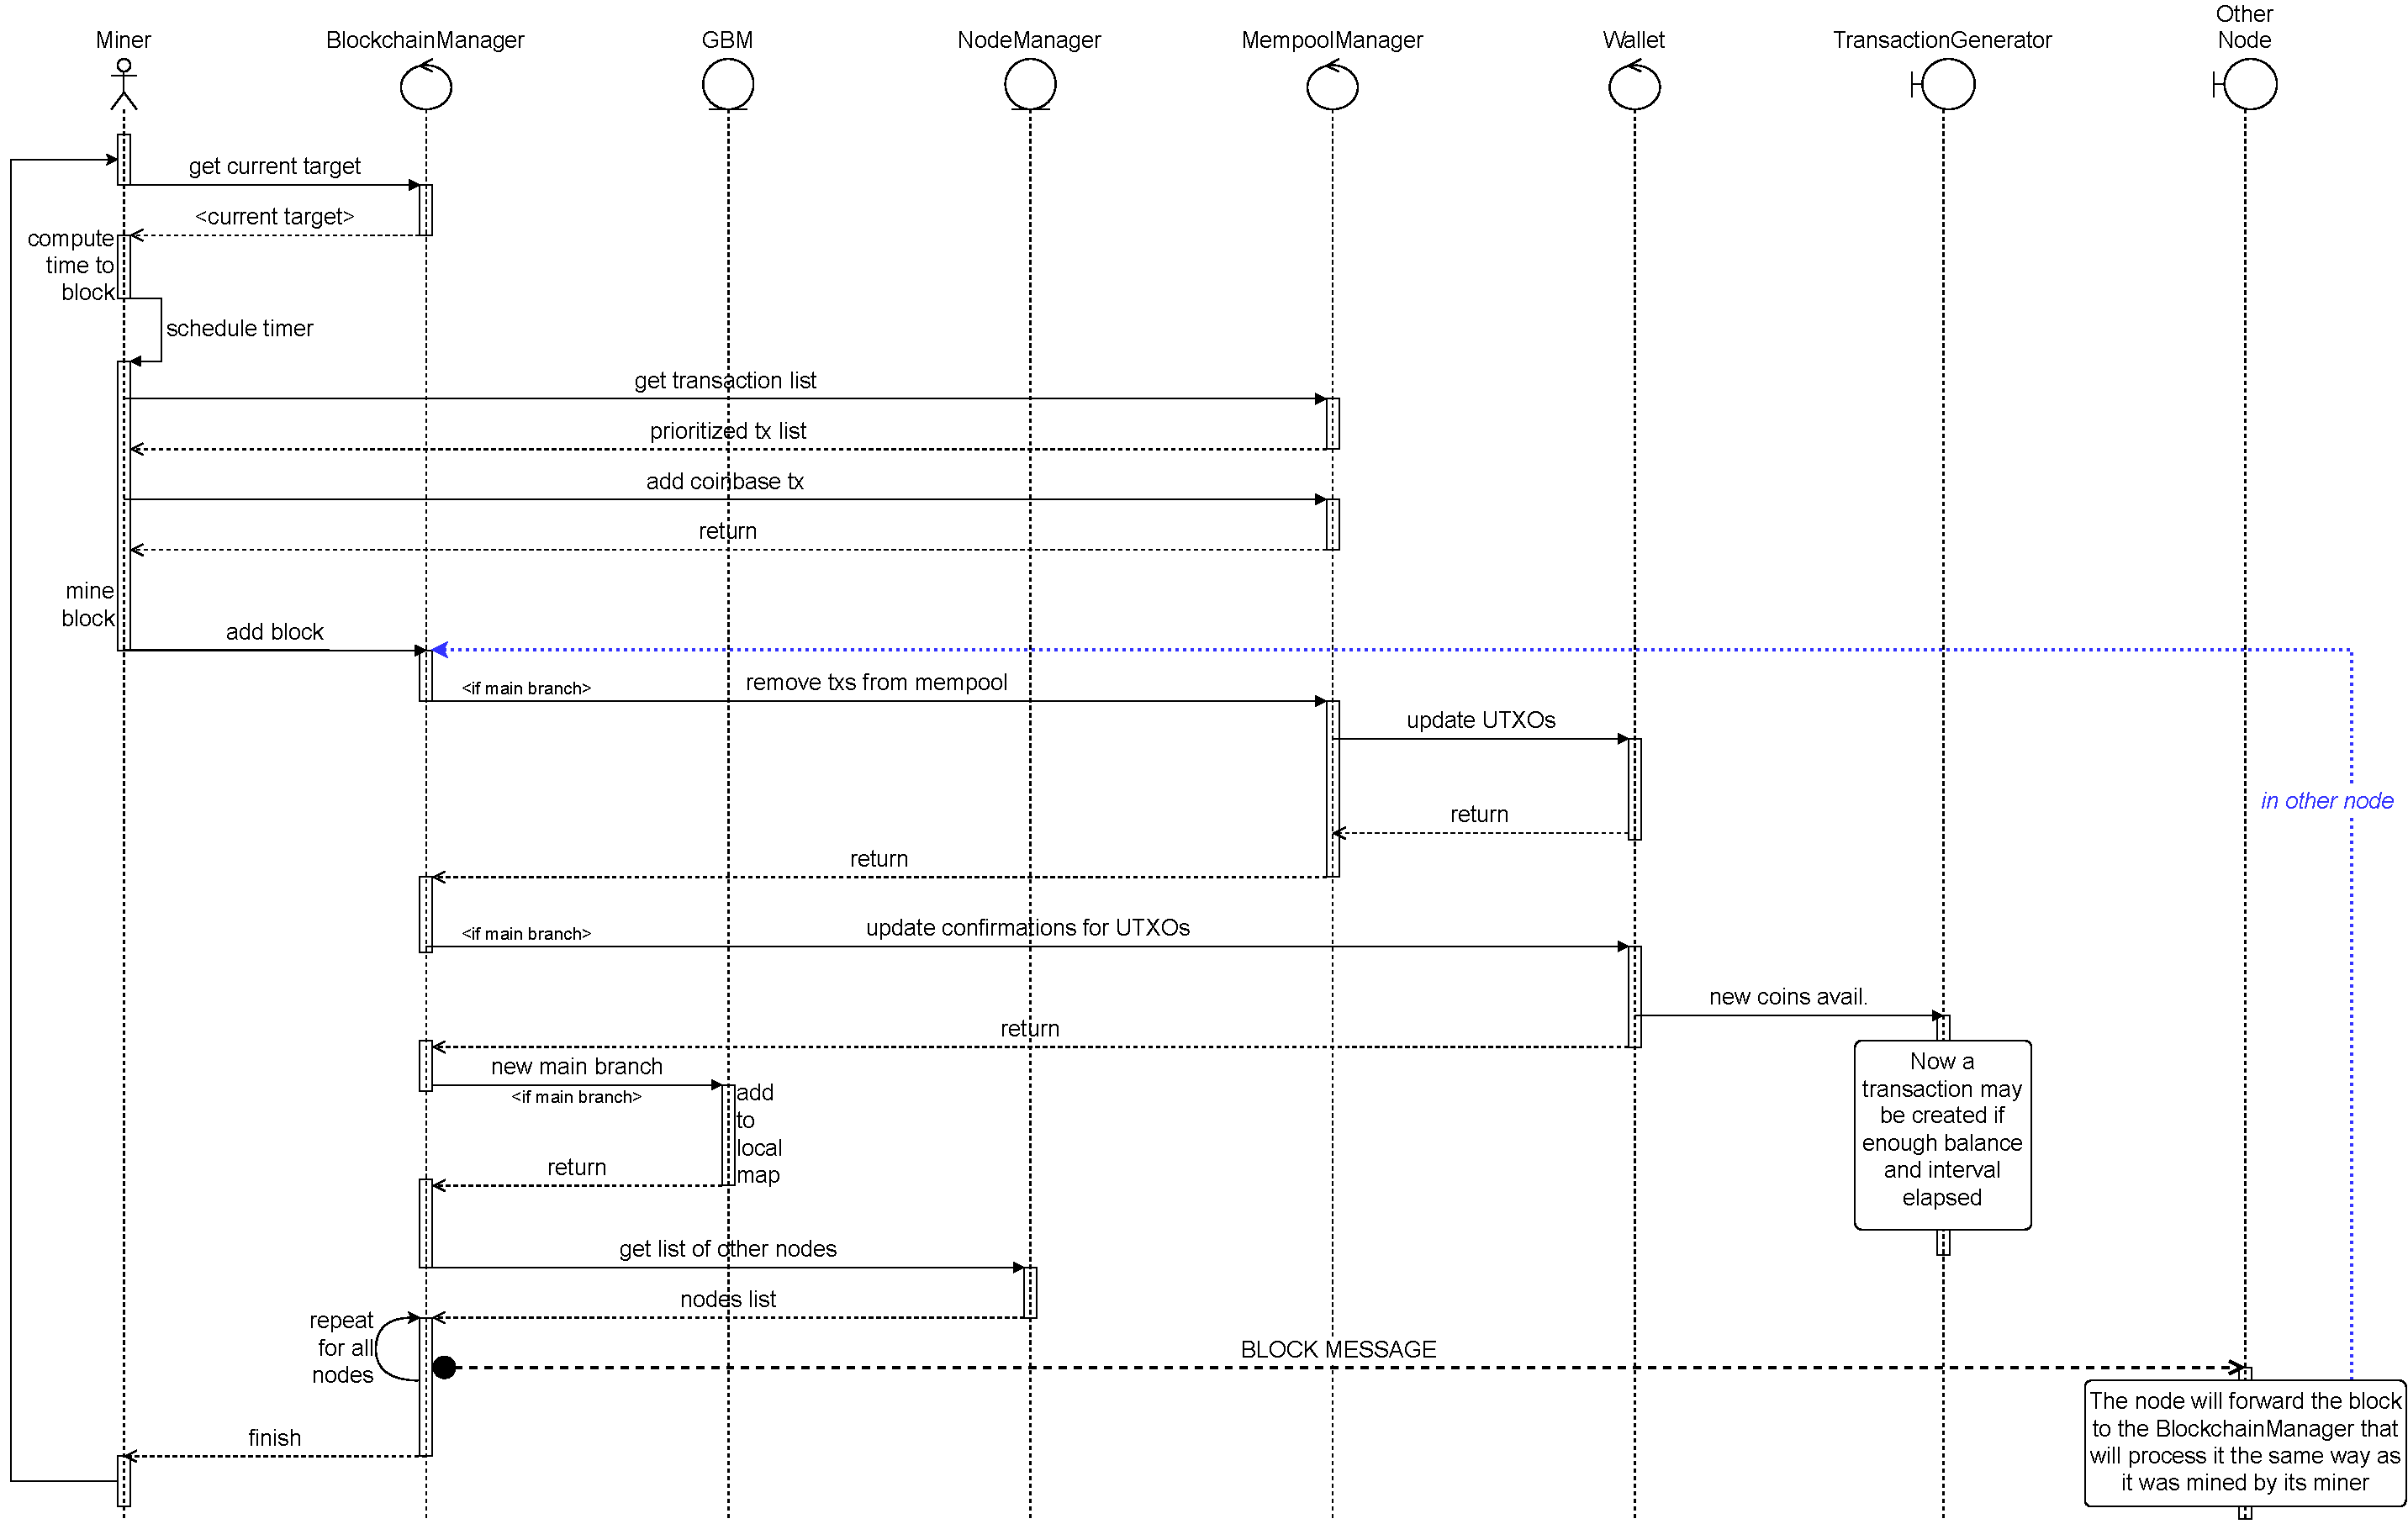
\includegraphics[width=\textheight,height=0.58\textwidth,keepaspectratio]{img/mining-sequence}
	\caption{UML sequence diagram illustrating the mining
	process.}\label{fig:mining-sequence}
\end{sidewaysfigure}

\begin{sidewaysfigure}
	\centering
	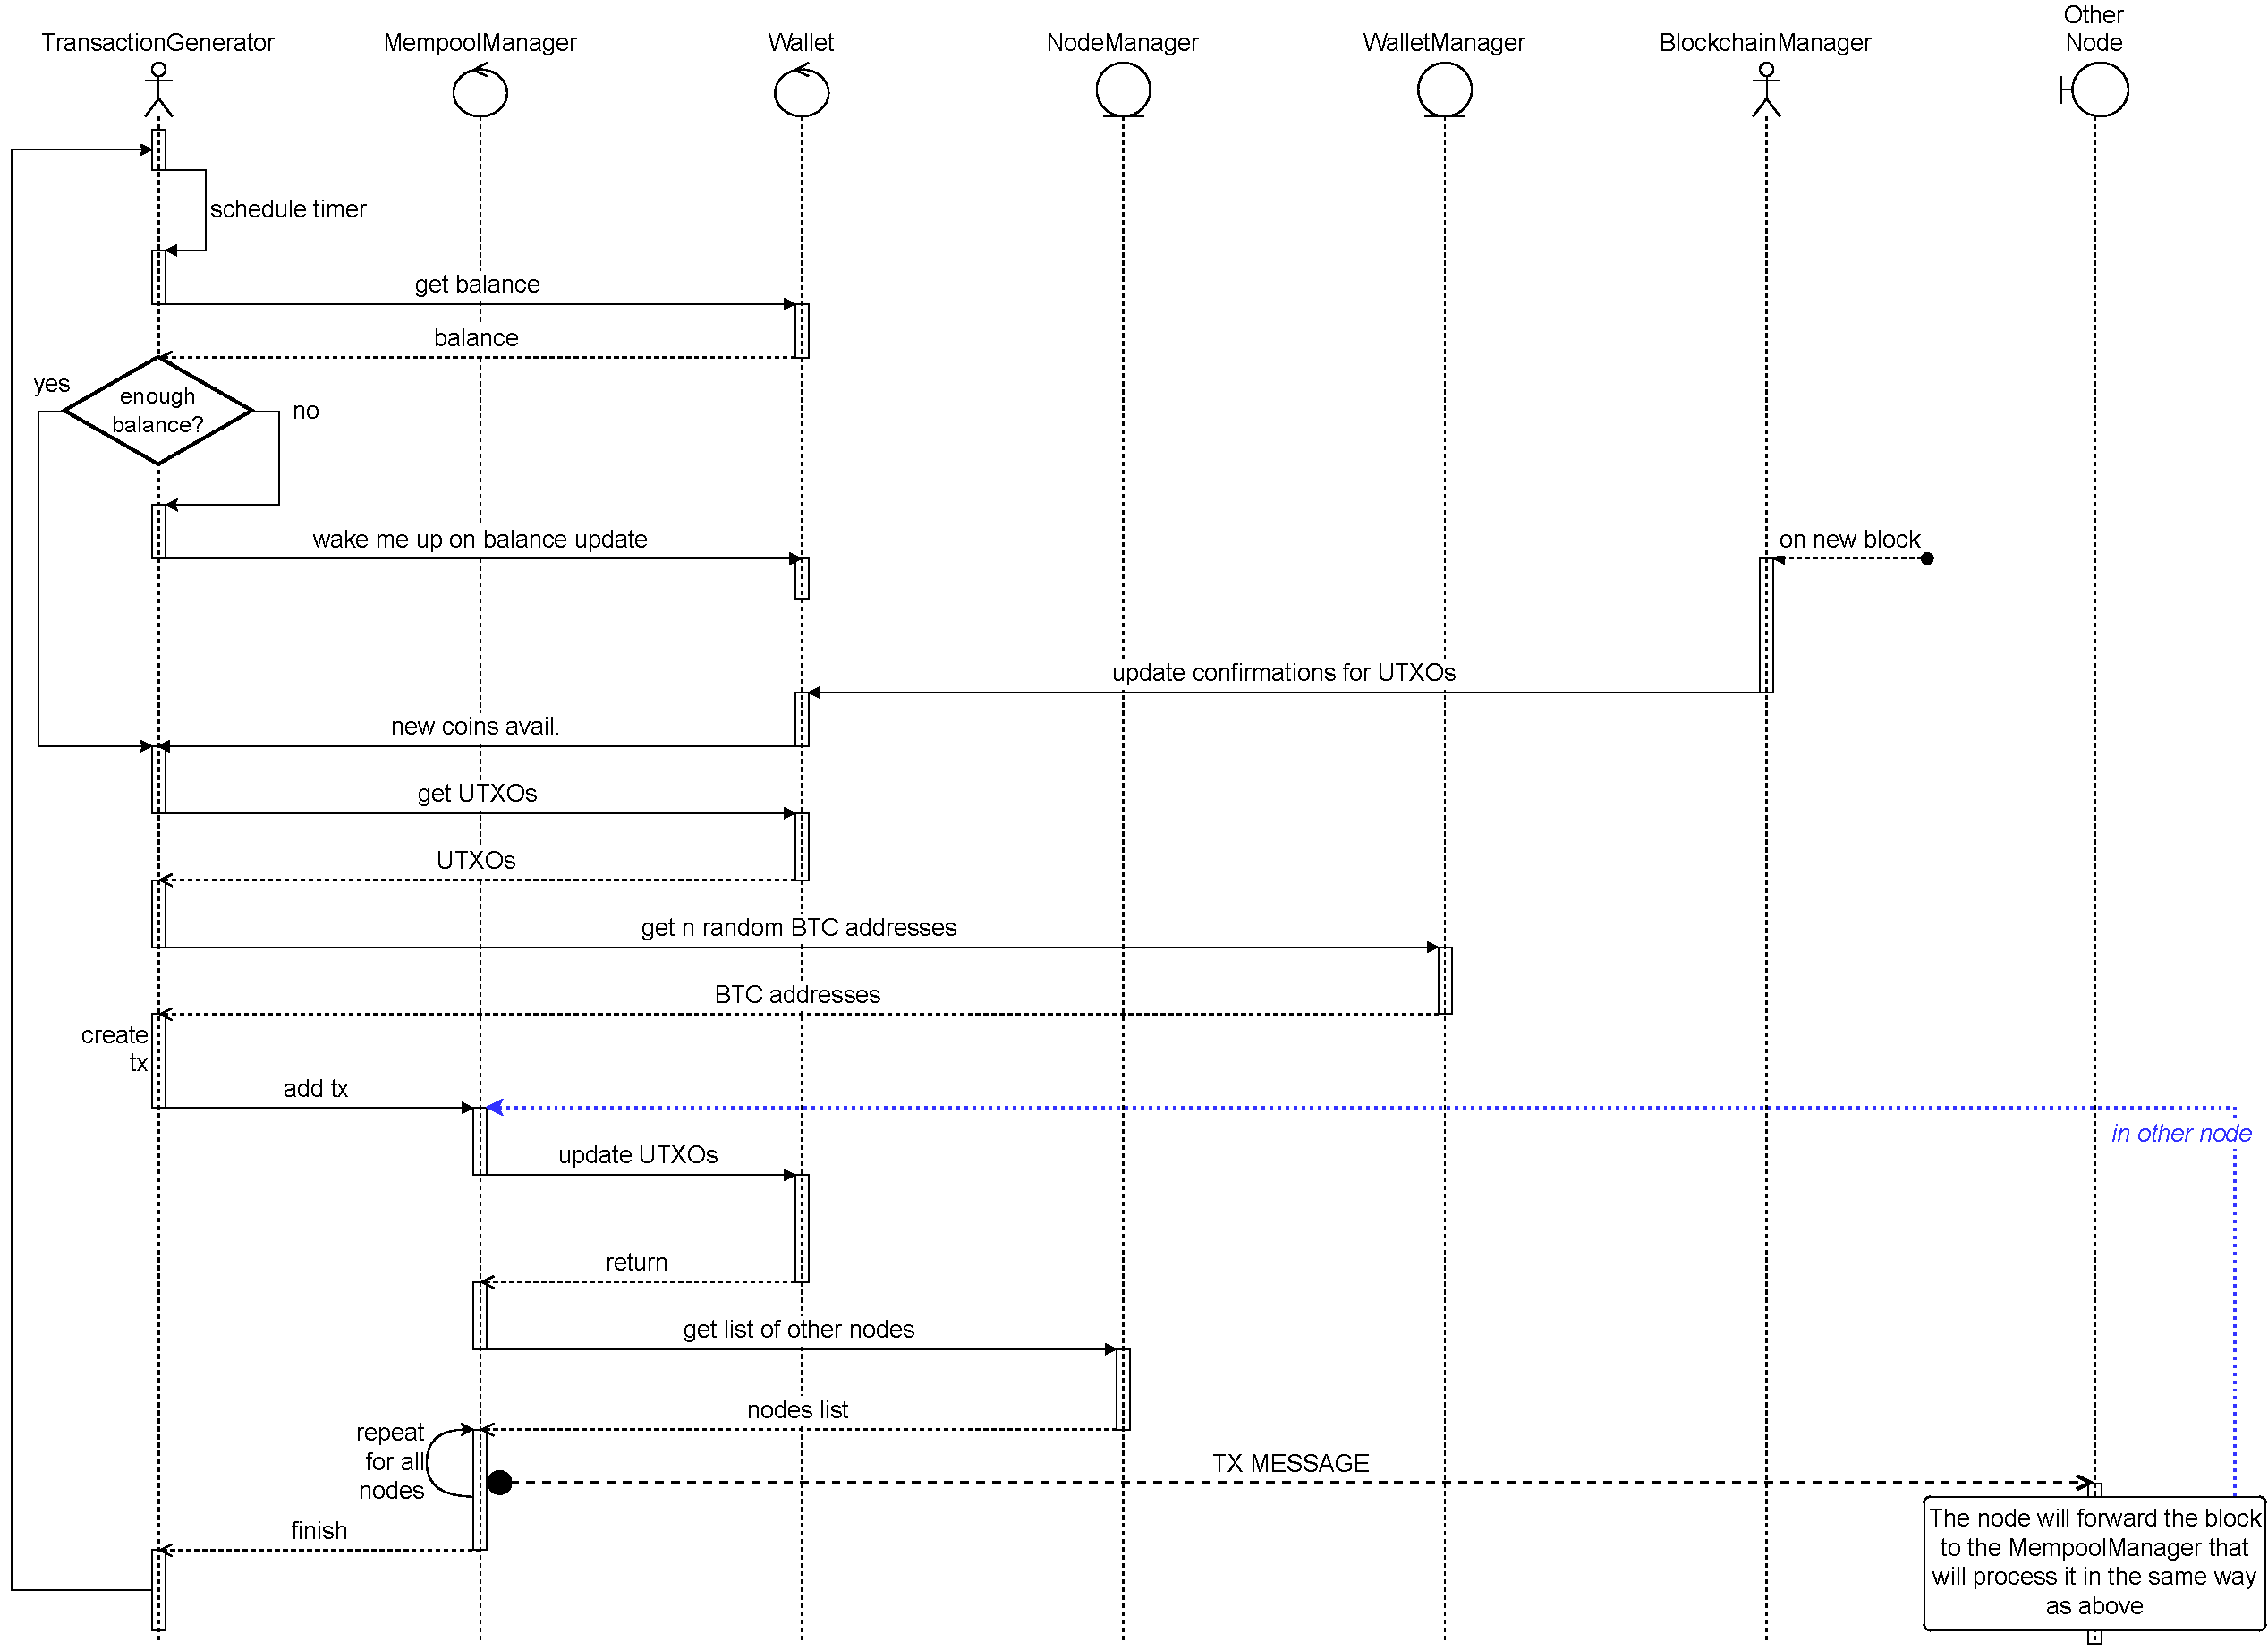
\includegraphics[width=\textheight,height=0.58\textwidth,keepaspectratio]{img/txgen-sequence}
	\caption{UML sequence diagram illustrating the transaction generation
	process.}\label{fig:txgen-sequence}
\end{sidewaysfigure}
